\documentclass[12pt, letterpaper]{article}

\usepackage{graphicx}
\graphicspath{ {images/} }
\usepackage[letterpaper, margin=1in]{geometry}
\usepackage{indentfirst}
\usepackage{secdot}
%\usepackage[toc,page]{appendix}
\usepackage{tocloft}
\usepackage{tabularx}
%\renewcommand{\baselinestretch}{1.9}
\usepackage{setspace}
\usepackage{float}
\doublespacing

\newcommand{\companyname}{Veg-To-Go}

\begin{document}

\title{\companyname{},\textsuperscript{\textregistered} Food Truck\\ Marketing Plan}
\author{Zach Pratt}
\maketitle

\newpage

\renewcommand\contentsname{Table of Contents}
\renewcommand{\cftsecleader}{\cftdotfill{\cftdotsep}}
\tableofcontents

\newpage

\section{Executive Summary}
Veg-To-Go is an upcoming mobile food venue serving a hearty and filling menu of plant based, animal and animal product free comfort food.  While the trend of food trucks, tents, and truck bed barbeques is already prominent in Fort Wayne, there is still a lack in these existing businesses of concern for the ethics of food.

Veg-To-Go hopes to provide wholesome and filling plates of flavorful and saucy food at a bigger price-to-ounce ratio, ultimately giving customers more savory food for their dollar.  This plan hopes to show that this will result in a bigger profit margin, saving the company money by eliminating expensive animal products and using simple frozen and fresh ingredients combined with proven methods of boosting savories using spices and herbs.

Building on this mission to completely satisfy Fort Wayne street food customers with cheap, generous, and healthy food, Veg-To-Go will begin by incrementally building its customer base.  The company will start by purchasing a minimal setup of a small flattop grill and source its frozen and dry ingredients from local warehouse and bulk sections. Produce will be purchased locally and fresh when possible.  The company will attend weekly farmers markets and set up outside bars throughout the week when possible.  After an initial trial phase and the establishment of a solid customer base, the company will purchase a dedicated food truck or other mobile venue to expand its existing business.

\section{Situation Analysis}
This situation analysis will demonstrate the current state of \companyname{} by examining the business environment through a SWOT analysis and detailed examination of the industry, competitors, company, and consumers.

\subsection{SWOT Analysis}
Figure \ref{SWOT} shows the factors affecting the market opportunities for \companyname{}.  This table highlights the efforts by the company to prepare to enter the local market.
\singlespacing
\begin{figure}
    \caption{SWOT Analysis for \companyname{}}
    \begin{center}
        \bgroup
        \def\arraystretch{1.5}%  1 is the default, change whatever you need
        \begin{tabularx}{\textwidth}{|X X X|}
            \hline
            Internal Factors & Strengths & Weaknesses\\
            \hline
            Management & Management has education in business and culinary arts & Inexperienced in business management\\
            \hline
            Offerings & Completely unique product to the local market & May be perceived as more light-weight or bland\\
            \hline
            Marketing & Continuous advertising via branding on food truck & Limited budget\\
            \hline
            Personnel & Small team, easy to communicate & Limited budget for additional help\\
            \hline
            Finance & Small startup cost & No proven growth\\
            \hline
            Manufacturing & Cheap to produce dishes & Limited work area\\
            \hline
            R\&D & Can be accomplished with limited resources & No formal process\\
            \hline
            \hline
            External Factors & Opportunities & Threats \\
            \hline
            Consumer/Social & Large potential dual market between farmer's markets and hungry bar-goers & Competitors have established relationship with partner businesses \\
            \hline
            Competitive & Only Fort Wayne vegan mobile food & Many bars have a food truck with regular customers \\
            \hline
            Technological & Can develop own website and app & Competitors have better equipment \\
            \hline
            Economic & Low cost, high customer value & Existing local company's already have capital \\
            \hline
            Legal/Regulatory & Already Serv-Safe certified & Local street food permit must be acquired \\
            \hline
        \end{tabularx}
        \egroup
        \label{SWOT}
    \end{center}
\end{figure}
\doublespacing

\subsection{Industry Analysis: Trends in Mobile Food Venues}
According the National Restaurant Association , the annual US food truck revenue is 2.7 billion dollars annually and rising. \cite{ibis1} With this kind of opportunity, it comes as no surprise
that many local entrepreneurs have begun to emerge. According to the Fort Wayne Food Truck association, there are over 51 food trucks, 14 organized under the association and 37 unorganized or non-affiliated trucks. \cite{fwfta}
\subsection{Competitor Analysis: Local Food Trucks}

\subsection{Company Analysis}
\subsection{Customer Analysis}
\subsubsection{Customer Characteristics}
\subsubsection{Health and Nutrition Concerns}

\section{Market-Product Focus}
Lorem ipsum dolor sit amet, consectetur adipiscing elit. Aenean fringilla sem et suscipit dapibus. Quisque a pulvinar mi, nec aliquet metus. Curabitur hendrerit porttitor purus. Phasellus a est nec ante pellentesque maximus. Mauris commodo enim risus, eget porttitor odio pharetra ac. Nullam elementum congue enim eget facilisis. Mauris lacus urna, bibendum ut venenatis fringilla, varius ac tellus. Curabitur venenatis rutrum nunc. Mauris in porttitor justo. Phasellus in vulputate eros. Mauris maximus diam eu tortor mattis, sed imperdiet dui rhoncus. Morbi ultrices maximus metus sed eleifend. Maecenas vestibulum in nibh efficitur imperdiet. Curabitur finibus tempor vehicula. Praesent pellentesque id justo eget blandit. Maecenas id odio nulla.
\subsection{Marketing and Product Objectives}
Sed vel sagittis nisi. Donec auctor eu est sed maximus. Aenean pharetra tincidunt ipsum, at rhoncus ipsum ullamcorper at. Nulla fringilla ligula nec risus maximus, ac gravida lorem pellentesque. Fusce vehicula malesuada fringilla. Nunc iaculis, lectus non faucibus dapibus, elit sapien hendrerit ipsum, id vehicula odio lacus ornare neque. Nullam in est pellentesque, euismod turpis et, ultrices ante.
\subsubsection{Target Markets}
Maecenas laoreet, ante sit amet malesuada mattis, sem libero egestas magna, ut commodo velit quam ut magna. Phasellus in eros at mi gravida rutrum. Etiam volutpat imperdiet malesuada. Vestibulum consequat ipsum pharetra, mattis turpis ut, dignissim diam. Curabitur et egestas sem. Mauris eu dui arcu. Sed quis nisi purus. Sed vitae porttitor ligula. Donec interdum metus ac turpis luctus gravida. In ultrices sem vitae magna finibus, vel condimentum tortor volutpat. Aliquam erat volutpat. Maecenas laoreet lectus ac purus luctus, nec accumsan risus tempor. Phasellus turpis massa, varius vitae massa nec, elementum aliquet libero. Praesent egestas feugiat massa sed tincidunt. Fusce pulvinar aliquet velit, et vulputate ligula aliquam vel. Donec at suscipit quam.
\subsubsection{Points of Difference}
Suspendisse semper lectus in nulla luctus semper. Praesent a fermentum ipsum. Fusce eget cursus mauris, id finibus lectus. Ut erat velit, finibus molestie porttitor sit amet, tincidunt ac magna. Vestibulum a dui dolor. In ut ipsum est. Mauris dui felis, elementum et mauris quis, eleifend gravida enim. Fusce justo est, varius quis eleifend lacinia, semper ac enim. Curabitur lobortis lorem quis purus facilisis egestas. Praesent non leo non enim facilisis imperdiet.
\subsubsection{Positioning}
Suspendisse semper lectus in nulla luctus semper. Praesent a fermentum ipsum. Fusce eget cursus mauris, id finibus lectus. Ut erat velit, finibus molestie porttitor sit amet, tincidunt ac magna. Vestibulum a dui dolor. In ut ipsum est. Mauris dui felis, elementum et mauris quis, eleifend gravida enim. Fusce justo est, varius quis eleifend lacinia, semper ac enim. Curabitur lobortis lorem quis purus facilisis egestas. Praesent non leo non enim facilisis imperdiet.

\section{Marketing Program Strategy and Tactics}
\subsection{Product Strategy}
Local produce will be purchased when possible, resulting in a slightly seasonal and varied product. Bulk herbs and spices will be purchased through local and on-line sources, allowing a predictable and constant flavor in each dish.

Components will be assembled off-site in advance where applicable, saving assembly time and improving delivery time and order fulfillment on-site. Examples include: rice cooked for the day, sauces prepped and stored, and vegetables cut in advance, preferably packaged in weighed portions for each dish.
\subsection{Price Strategy}
All entree dishes will be equally priced at \$8 a plate, and sides at \$4 per serving. Entrees will contain between 12 and 16 ounces of food at \$.50 an ounce. The ingredients for each dish will cost at most \$.15 an ounce, with the bulk of the meal consisting of rice (approximately \$.03 an ounce \cite{costs}) and the rest mixed vegetables (\$.10 and ounce) with dried herbs and spices (\$.02 an ounce), yielding approximately a desirable 3 times markup. A similar markup is applied to the sides.  These prices will remain constant the first three years.
\subsection{Promotion Strategy}
Promotion is to be done as the budget allows, using roughly 2\% of quarterly revenue and consists of food giveaways and graphical posters strategically placed in bars and at schools.  Customers may also check in through Facebook, Google+ or the Veg-To-Go mobile app to get 10\% off their meal.

Promotion the first year will focus heavily on the Mexican and Chinese dishes at first (see Figure \ref{products}), featuring the potatoes as a side. After the first year, the Italian entree will be added to the promotional mix.

The first target market will consist of adults 18-35 at nighttime venues and will primarily appeal to a desire to eat a filling meal while out with friends and secondarily appeal to a sense of doing good for the environment by eating sustainably.

Sign-age and graphical promotion will begin to expand the second year to target families at daytime venues.  Advertising during the day will incorporate imagery and phrasing to reflect eating hearty and healthy in the context of a family outing.
\subsection{Place (Distribution) Strategy}
Relationships are established with local bars, nightlife locations, and farmer's markets during the first year.  Some of the promotional budget will be used to provide meal trade and incentives to establish rapport with these partner businesses.  In addition, advertising may be offering through the company's mobile app and social media outlets for partners, which will reduce some cost in forming these alliances.

The second and third year will consist of maintaining a consistent presence and expanding to the company's secondary target market (families) by offering free 1/2 size meals for children 12 and under at daytime venues.

\section{Financial Projections}
\subsection{Three-Year Projections}

\begin{figure}[H]
	\caption{Sales and Expenses for \companyname{}}
	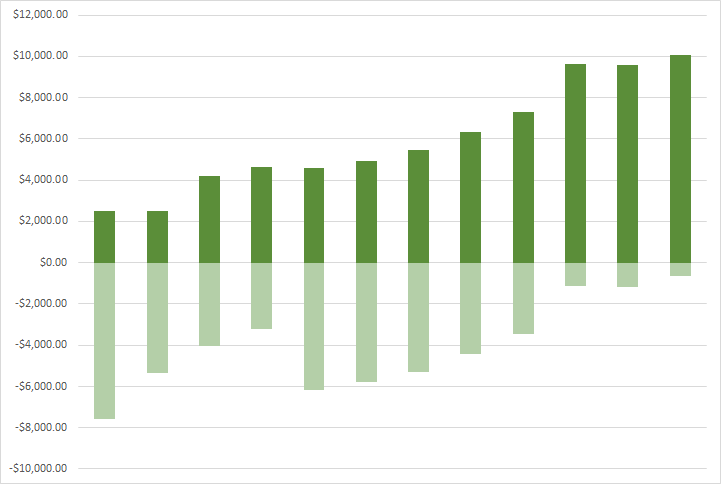
\includegraphics[width=\textwidth]{SalesAndExpenses}
\end{figure}

\begin{figure}[H]
	\label{products}
	\caption{Sales for \companyname{}}
	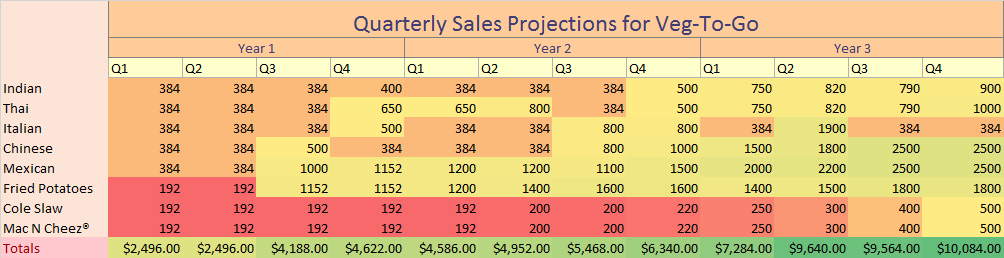
\includegraphics[width=\textwidth]{SalesNumbers}
\end{figure}

\begin{figure}[H]
	\caption{Expenses for \companyname{}}
	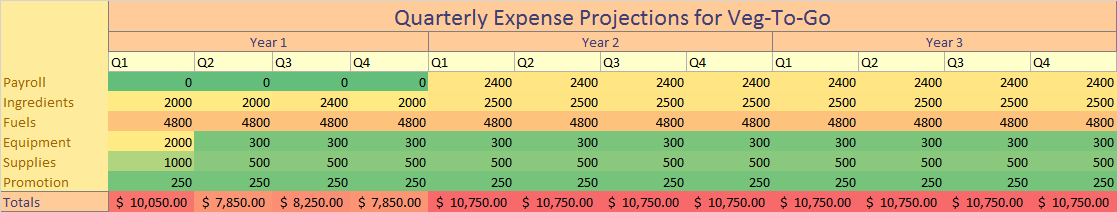
\includegraphics[width=\textwidth]{ExpensesNumbers}
\end{figure}

\begin{figure}[H]
	\caption{Total 3-Year Profit for \companyname{}}
	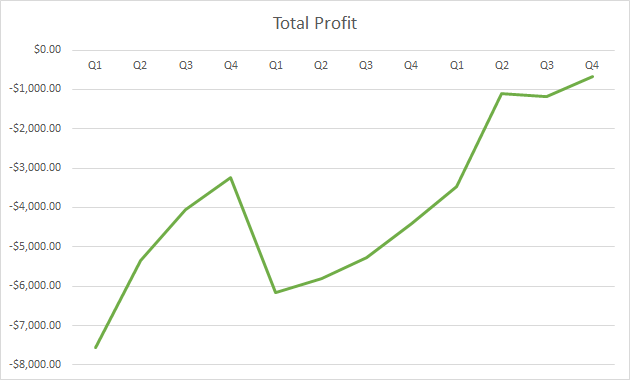
\includegraphics[width=\textwidth]{TotalProfit}
\end{figure}

\section{Implementation Plan}
The company will initially purchase a graphical tent under which the food is cooked and served truck-side.  A single induction burner serves as the heating elements for pre-prepared, fresh ingredients.  The dishes mainly consist of a sauce that dictates the cuisine, combined with veggies and served over white rice.  The setup and costs are kept to a minimum, but the flavor is boosted using lightweight dried and fresh herbs and spices and international inspiration.

The company will be ran by a single owner, and after the first year will hire an employee for 5 hours a day.

\section{Evaluation}
Lorem ipsum dolor sit amet, consectetur adipiscing elit. Aenean fringilla sem et suscipit dapibus. Quisque a pulvinar mi, nec aliquet metus. Curabitur hendrerit porttitor purus. Phasellus a est nec ante pellentesque maximus. Mauris commodo enim risus, eget porttitor odio pharetra ac. Nullam elementum congue enim eget facilisis. Mauris lacus urna, bibendum ut venenatis fringilla, varius ac tellus. Curabitur venenatis rutrum nunc. Mauris in porttitor justo. Phasellus in vulputate eros. Mauris maximus diam eu tortor mattis, sed imperdiet dui rhoncus. Morbi ultrices maximus metus sed eleifend. Maecenas vestibulum in nibh efficitur imperdiet. Curabitur finibus tempor vehicula. Praesent pellentesque id justo eget blandit. Maecenas id odio nulla.

Sed vel sagittis nisi. Donec auctor eu est sed maximus. Aenean pharetra tincidunt ipsum, at rhoncus ipsum ullamcorper at. Nulla fringilla ligula nec risus maximus, ac gravida lorem pellentesque. Fusce vehicula malesuada fringilla. Nunc iaculis, lectus non faucibus dapibus, elit sapien hendrerit ipsum, id vehicula odio lacus ornare neque. Nullam in est pellentesque, euismod turpis et, ultrices ante.

Maecenas laoreet, ante sit amet malesuada mattis, sem libero egestas magna, ut commodo velit quam ut magna. Phasellus in eros at mi gravida rutrum. Etiam volutpat imperdiet malesuada. Vestibulum consequat ipsum pharetra, mattis turpis ut, dignissim diam. Curabitur et egestas sem. Mauris eu dui arcu. Sed quis nisi purus. Sed vitae porttitor ligula. Donec interdum metus ac turpis luctus gravida. In ultrices sem vitae magna finibus, vel condimentum tortor volutpat. Aliquam erat volutpat. Maecenas laoreet lectus ac purus luctus, nec accumsan risus tempor. Phasellus turpis massa, varius vitae massa nec, elementum aliquet libero. Praesent egestas feugiat massa sed tincidunt. Fusce pulvinar aliquet velit, et vulputate ligula aliquam vel. Donec at suscipit quam.

Suspendisse semper lectus in nulla luctus semper. Praesent a fermentum ipsum. Fusce eget cursus mauris, id finibus lectus. Ut erat velit, finibus molestie porttitor sit amet, tincidunt ac magna. Vestibulum a dui dolor. In ut ipsum est. Mauris dui felis, elementum et mauris quis, eleifend gravida enim. Fusce justo est, varius quis eleifend lacinia, semper ac enim. Curabitur lobortis lorem quis purus facilisis egestas. Praesent non leo non enim facilisis imperdiet.

Proin feugiat, augue vitae sagittis ullamcorper, diam sem tincidunt lectus, non elementum dolor nisl a tortor. Duis sed diam tincidunt dui pharetra finibus vitae nec tellus. Etiam sed nibh commodo, consectetur enim et, tempor lacus. Fusce eu porttitor tellus. Aenean egestas mi eu ultrices fermentum. Duis euismod vulputate massa nec dignissim. Aenean viverra at velit quis viverra.

\newpage

\begin{thebibliography}{9}

    \bibitem{ibis1}
        Food Trucks in the US: Market Research Report. Retrieved October 10, 2015, from http://www.ibisworld.com/industry/food-trucks.html
    \bibitem{paste}
        Food Trucks in the US: Market Research Report. Retrieved October 10, 2015, from http://www.ibisworld.com/industry/food-trucks.html        
    \bibitem{fwfta}
        Food Trucks in the US: Market Research Report. Retrieved October 10, 2015, from http://www.ibisworld.com/industry/food-trucks.html
    \bibitem{costs}
        Average Retail Food and Energy Prices, U.S. and Midwest Region. (n.d.). Retrieved November 14, 2015, from http://www.bls.gov/regions/mid-atlantic/data/AverageRetailFoodAndEnergyPrices\_USandMidwest\_Table.htm

\end{thebibliography}

\newpage

%\begin{appendices}
%\end{appendices}

\end{document}
